
本节中,我们将了解Clang的AST内存表示和基本API的用法。本节的第一部分将提供Clang AST的层次结构的高级概述;第二部分将关注一个更具体的主题——关于Clang AST中的类型表示;最后一部分将展示AST匹配器的基本用法,这在编写AST插件时非常有用。

\subsubsubsection{7.2.1\hspace{0.2cm}Clang的AST内存表示}

在Clang中,AST的内存表示为一个层次结构,类似于C族语言程序的语法结构。从最顶层开始,这里有两个类值得一提:

\begin{itemize}
\item \texttt{TranslationUnitDecl}: 该类表示一个输入源文件,也称为翻译单元(大多数情况下)。包含所有顶级声明——举几个例子,全局变量、类和函数——作为子声明,其中每个顶级声明都有自己的子树,子树递归地定义AST的其余部分。

\item \texttt{ASTContext}: 顾名思义,这个类跟踪所有AST节点和来自输入源文件的其他元数据。如果有多个输入源文件,每个都有自己的\texttt{TranslationUnitDecl},但都共享相同的\texttt{ASTContext}。
\end{itemize}

除了结构之外,AST的主体(AST节点)还可以进一步分为三个主要类别:\textbf{声明}、\textbf{语句}和\textbf{表达式}。这些类别中的节点分别由派生自\texttt{Decl}、\texttt{Expr}和\texttt{Stmt}类的子类表示。在后续的部分中,我们将介绍这些内存中的AST表示。

\hspace*{\fill} \\ %插入空行
\noindent
\textbf{声明}

语言结构,如变量声明(全局和局部)、函数和结构/类声明,都是由\texttt{Decl}的子类表示。虽然我们不打算在这里详细介绍每一个子类,但下图展示了C/C++中常见的声明结构和它们对应的AST类:

\hspace*{\fill} \\ %插入空行
\begin{center}
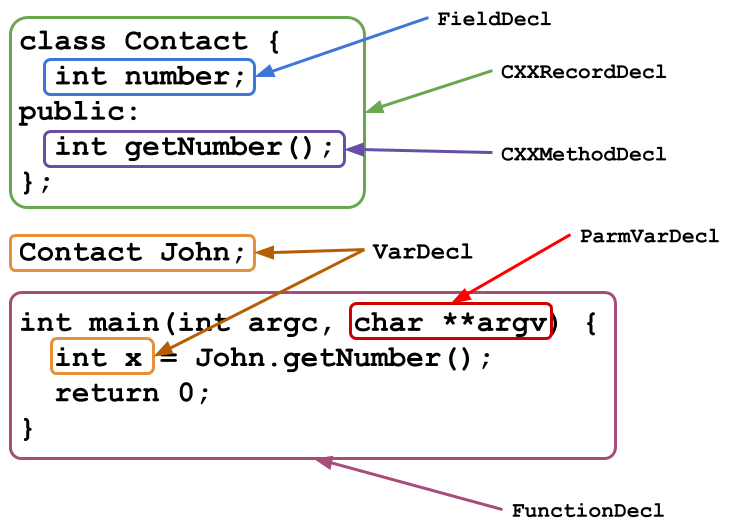
\includegraphics[width=0.7\textwidth]{content/2/chapter7/images/1.png}\\
图7.1 - C/C++中常见的声明及其AST类
\end{center}

在更具体的子类之间,比如\texttt{FunctionDecl}和\texttt{Decl},有几个重要的\textit{抽象}类代表特定的语言概念:

\begin{itemize}
\item \texttt{NamedDecl}: 每个声明都有名称。
\item \texttt{ValueDecl}: 声明的实例可以是一个值,从而声明可以与类型信息相关联。
\item \texttt{DeclaratorDecl}: 对于每个声明(基本上是以\texttt{<类型和限定符> <标识符名称>}形式的语句),提供了除标识符之外的有关部件的额外信息。例如,提供对具有名称空间解析的内存对象的访问,该名称空间解析在声明器中充当了限定符。
\end{itemize}

要了解更多关于AST类的其他声明,可以在LLVM的官方API在线网站上浏览\texttt{Decl}的子类。

\hspace*{\fill} \\ %插入空行
\noindent
\textbf{语句}

程序中大多数表示\textit{动作}概念的指令都可以视为语句,并由\texttt{Stmt}的子类表示,包括\textit{表达式}(我们很快就会讲到)。除了命令式语句(如函数调用或返回站点)之外,\texttt{Stmt}还涵盖了结构概念,如\texttt{for}循环和\texttt{if}语句。下面这张图展示了C/C++中\texttt{Stmt}(表达式除外)表示的通用语言结构,及其对应的AST类:

\hspace*{\fill} \\ %插入空行
\begin{center}
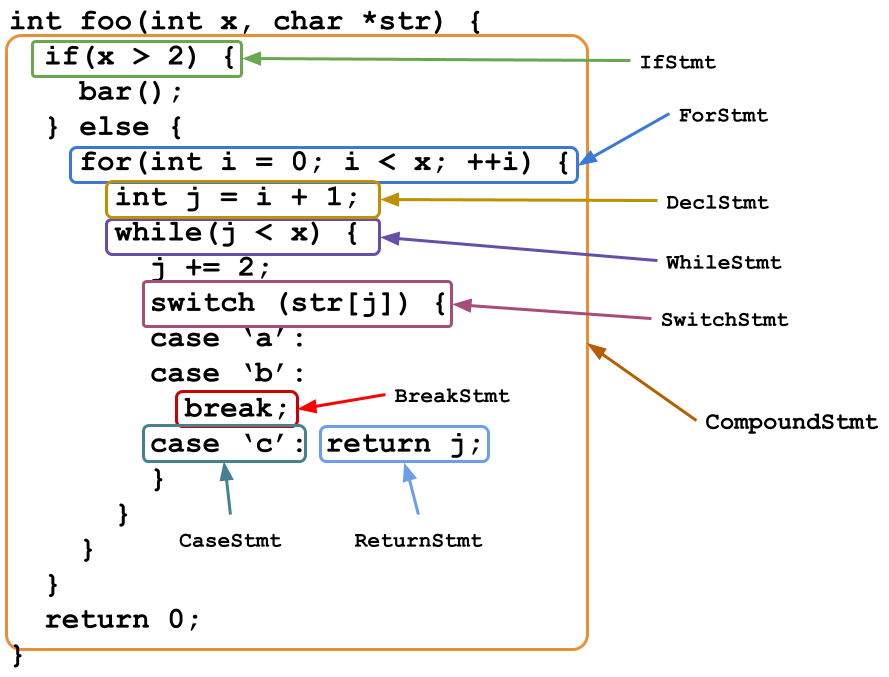
\includegraphics[width=0.8\textwidth]{content/2/chapter7/images/2.png}\\
图7.2 - C/C++及其AST类中的通用语句(表达式除外)
\end{center}

关于上图,有两点值得注意:

\begin{itemize}
\item \texttt{CompoundStmt}是一个包含多个语句的容器,不仅表示函数体,而且基本上表示由大括号(\texttt{'\{','\}'})包围的任何代码块。因此,尽管由于缺少空间在前面的图中没有显示,但\texttt{IfStmt}、\texttt{ForStmt}、\texttt{WhileStmt}和\texttt{SwitchStmt}都有一个表示主体的\texttt{CompoundStmt}子节点。

\item \texttt{CompoundStmt}中的声明使用\texttt{DeclStmt}节点包装,其中真正的\texttt{Decl}实例是它的子节点。这是一个更简单的AST设计。
\end{itemize}

语句是C/C++程序中最流行的指令之一。值得注意的是,许多语句都组织在一个层次结构中(例如,\texttt{ForStmt}及其循环体),因此在找到所需的\texttt{Stmt}节点之前,可能需要执行额外的步骤来深入这个层次结构。

\hspace*{\fill} \\ %插入空行
\noindent
\textbf{表达式}

Clang AST中的表达式是一种特殊的语句。与其他语句不同,表达式总是生成\textit{值}。例如,期望一个简单的算术表达式3 + 4生成一个整数值。Clang AST中的所有表达式都由\texttt{Expr}的子类表示。下面这张图展示了C/C++中常用的\texttt{Expr}表示的语言结构及其对应的AST类:

\hspace*{\fill} \\ %插入空行
\begin{center}
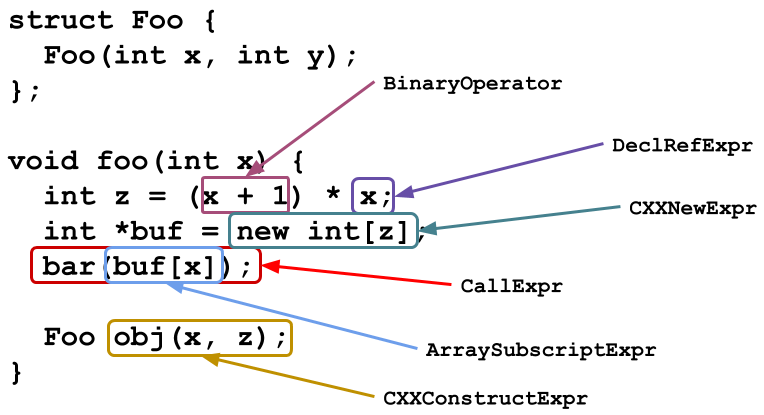
\includegraphics[width=0.7\textwidth]{content/2/chapter7/images/3.png}\\
图7.3 - C/C++中的常见表达式及其AST类
\end{center}

一个重要的\texttt{Expr}类是\texttt{DeclRefExpr},表示符号引用的概念。可以使用\texttt{DeclRefExpr::getDecl()}来检索引用符号的\texttt{Decl}对象。像这样方便的符号信息只有在生成AST之后才会出现,所以这就是为什么人们总是建议在AST上实现静态分析逻辑,而不是在更原始的形式上(例如,在解析器中)。

另一个有趣的\texttt{Expr}类(由于缺少空格,上图中没有突出显示)是\texttt{ParenExpr},它表示包围表达式的圆括号。例如,在前面的图中,(x + 1)是一个\texttt{ParenExpr},它带有一个\texttt{BinaryOperator},将x + 1表示为它的子元素。

\subsubsubsection{7.2.2\hspace{0.2cm}Clang AST中的类型}

类型系统是现代编译器中最重要的组件之一,特别是对于C/C++这样的静态类型语言。类型检查确保输入源代码是格式良好的(某种程度上),并在编译时捕获尽可能多的错误。虽然不需要在Clang中自己做类型检查,检查的操作由Sema子系统完成(在第5章中介绍了这个子系统)。在处理AST时,可能需要利用这些信息。让我们了解如何在Clang AST中建模类型。

\hspace*{\fill} \\ %插入空行
\noindent
\textbf{核心类型}

Clang AST类型系统的核心是\texttt{clang::Type}类。输入代码中的每种类型——包括\texttt{int}这样的基本类型和struct/class这样的用户定义类型——都由一个单例类型(更具体地说,是\texttt{Type}的\textit{子类})对象表示。

\begin{tcolorbox}[colback=blue!5!white,colframe=blue!75!black, fonttitle=\bfseries,title=术语]
\hspace*{0.7cm}本章的其余部分中,将调用输入源代码中的类型。
\end{tcolorbox}

单例是一种设计模式,它强制一个资源或抽象概念只能由一个内存对象表示。我们的例子中,源代码类型就是资源,所以对于每一种类型,您只能找到一个\texttt{Type}对象。这种设计的最大优点是,有一种更简单的方法来比较两个\texttt{Type}对象。假设有两个\texttt{Type}指针,通过对它们做简单的指针比较(非常快),就可以知道它们是否表示相同的源代码类型。

\begin{tcolorbox}[colback=blue!5!white,colframe=blue!75!black, fonttitle=\bfseries,title=单例设计的反例]
\hspace*{0.7cm}如果Clang AST中的\texttt{Type}不是使用单例设计,为了比较两个\texttt{Type}指针是否代表相同的源代码类型,需要检查它们指向的对象的内容,不过这是无效的。
\end{tcolorbox}

正如前面提到的,每个源代码类型实际上都由\texttt{Type}的子类表示。下面是一些常见的\texttt{Type}子类:

\begin{itemize}
\item \texttt{BuiltinType}: 基本类型,如\texttt{int}、\texttt{char}和\texttt{float}。

\item \texttt{PointerType}: 所有的指针类型,有一个名为\texttt{PointerType::getPointee()}的函数,用于检索它所指向的源代码类型。

\item \texttt{ArrayType}: 所有的数组类型。这里,还有其他更特定的数组的子类,这些数组要么是定长的,要么是变长的。

\item \texttt{RecordType}: 结构/类/联盟类型。它有一个名为\texttt{RecordType::getDecl()}的函数,用于检索底层的\texttt{RecordDecl}。

\item \texttt{FunctionType}: 用于表示函数的签名,用于表示函数的参数类型和返回类型(以及其他属性,比如调用约定)。

\end{itemize}

现在让我们继续讨论限定类型。

\hspace*{\fill} \\ %插入空行
\noindent
\textbf{限定类型}

对于刚接触Clang代码库的人来说,最令人困惑的事情是,许多地方使用\texttt{QualType}类,而不是\texttt{Type}的子类来表示源代码类型。\texttt{QualType}表示\textbf{限定类型}。它充当\texttt{Type}的包装器,以表示\texttt{const <type>}、\texttt{volatile <type>}和\texttt{restrict <type>*}。

要从类型指针创建\texttt{QualType},可以使用以下代码:

\begin{lstlisting}[style=styleCXX]
// If `T` is representing 'int'…
QualType toConstVolatileTy(Type *T) {
	return QualType(T, Qualifier::Const | Qualifier::Volatile);
} // Then the returned QualType represents `volatile const int`
\end{lstlisting}

在本节中,我们了解了Clang AST中的类型系统。现在让我们继续了解ASTMatcher——一种匹配模式的语法。

\subsubsubsection{7.2.3\hspace{0.2cm}ASTMatcher}

当处理程序的AST时——例如,检查是否有任何次优语法——搜索特定的AST节点\textit{模式}通常是第一步,是人们最常做的事情。利用在前一节中学到的知识,我们知道这种模式匹配可以通过通过AST节点的内存类API迭代来完成。例如,给定一个\texttt{FunctionDecl}(函数的AST类),可以使用下面的代码来确定函数体中是否有一个\texttt{while}循环,以及该循环的退出条件是否总是一个布尔值,或者说是否为\texttt{true}:

\begin{lstlisting}[style=styleCXX]
// `FD` has the type of `const FunctionDecl&`
const auto* Body = dyn_cast<CompoundStmt>(FD.getBody());
for(const auto* S : Body->body()) {
	if(const auto* L = dyn_cast<WhileStmt>(S)) {
		if(const auto* Cond = dyn_cast<CXXBoolLiteralExpr>
		(L->getCond()))
		if(Cond->getValue()) {
			// The exit condition is `true`!!
		}
	}
}
\end{lstlisting}

它创建了超过三层(缩进)的\texttt{if}来完成这样一个简单的检查。更不要说在实际情况中,我们需要在这些行之间插入更多的健全性检查!虽然Clang的AST设计并不难理解,但我们需要更简洁的语法来完成模式匹配工作。幸运的是,Clang已经提供了一个——\textbf{ASTMatcher}。

ASTMatcher是一个实用工具,可以通过干净、简洁和高效的\textbf{领域特定语言(DSL)}编写AST模式匹配逻辑。使用ASTMatcher,前面的代码中做相同的匹配只需要几行代码:

\begin{lstlisting}[style=styleCXX]
functionDecl(compountStmt(hasAnySubstatement(
  whileStmt(
    hasCondition(cxxBoolLiteral(equals(true)))))));
\end{lstlisting}

前面代码片段中的大多数指令都非常简单:函数调用,如\texttt{compoundStmt(…)}和\texttt{whileStmt(…)},检查当前节点是否匹配特定的节点类型。这里,这些函数调用中的参数要么表示其子树上的模式匹配器,要么检查当前节点的其他属性。还有其他一些指令用于表示限定概念(例如,\textit{对于这个循环体中的所有子语句,都存在一个返回值}),例如\texttt{hasAnySubstatement(…)},以及用于表示数据类型和常量值的指令,例如\texttt{cxxBoolLiteral(equals(true))}的组合。

简而言之,使用ASTMatcher可以使您的模式匹配逻辑更具表现力。本节中,我们展示了这个优雅的DSL的基本用法。

\hspace*{\fill} \\ %插入空行
\noindent
\textbf{遍历AST}

在深入研究核心语法之前,我们先了解ASTMatcher是如何遍历AST的;以及在匹配过程完成后,是如何将结果返回给用户的。

\texttt{MatchFinder}是模式匹配过程中常用的驱动程序,基本用法非常简单:

\begin{lstlisting}[style=styleCXX]
using namespace ast_matchers;
…
MatchFinder Finder;
// Add AST matching patterns to `MatchFinder`
Finder.addMatch(traverse(TK_AsIs, pattern1), Callback1);
Finder.addMatch(traverse(TK_AsIs, pattern2), Callback2);
…
// Match a given AST. `Tree` has the type of `ASTContext&`
// If there is a match in either of the above patterns,
// functions in Callback1 or Callback2 will be invoked
// accordingly
Finder.matchAST(Tree);

// …Or match a specific AST node. `FD` has the type of
// `FunctionDecl&`
Finder.match(FD, Tree);
\end{lstlisting}

\texttt{pattern1}和\texttt{pattern2}是由DSL构造的模式对象,如前面所示。更有趣的是\texttt{traverse}函数和\texttt{TK\_AsIs}参数。\texttt{traverse}函数是模式匹配DSL的一部分,但它不是表示模式,而是描述遍历AST节点的操作。在此之上,\texttt{TK\_AsIs}参数可以表示\textit{遍历模式}。

当我们在本章前面展示了以文本格式转储AST的命令行标志(\texttt{-Xclang -ast-dump})时,您可能已经发现许多隐藏的AST节点会插入到树中,以帮助处理程序的语义,而不表示为程序员编写的真正代码。例如,\texttt{ImplicitCastExpr}会插入到很多地方,以确保程序的类型正确性。在编写模式匹配逻辑时,处理这些节点可能是一种痛苦的体验。因此,遍历函数提供了另一种简化的遍历树的方法。假设我们有以下源码:

\begin{lstlisting}[style=styleCXX]
struct B {
	B(int);
};
B foo() { return 87; }
\end{lstlisting}

当传递\texttt{TK\_AsIs}作为遍历的第一个参数时,其会先观察树,就像\texttt{-ast-dump}那样:

\begin{tcblisting}{commandshell={}}
FunctionDecl
`-CompoundStmt
  `-ReturnStmt
    `-ExprWithCleanups
      `-CXXConstructExpr
        `-MaterializeTemporaryExpr
          `-ImplicitCastExpr
            `-ImplicitCastExpr
              `-CXXConstructExpr
                `-IntegerLiteral 'int' 87
\end{tcblisting}

然而,通过将\texttt{TK\_IgnoreUnlessSpelledInSource}作为第一个参数,观察到的树等于如下所示:

\begin{tcblisting}{commandshell={}}
FunctionDecl
`-CompoundStmt
  `-ReturnStmt
    `-IntegerLiteral 'int' 87
\end{tcblisting}

顾名思义,\texttt{TK\_IgnoreUnlessSpelledInSource}只访问在源码中真正显示的节点。因为我们不再需要担心AST的本质细节,所以这极大地简化了编写匹配模式的过程。

另一方面,第一个代码中的\texttt{Callback1}和\texttt{Callback2}是\texttt{MatchFinder::MatchCallback}对象,它们描述了当有匹配时要执行的操作。下面是\texttt{MatchCallback}实现的框架:

\begin{lstlisting}[style=styleCXX]
struct MyMatchCallback : public MatchFinder::MatchCallback {
	void run(const MatchFinder::MatchResult &Result) override {
		// Reach here if there is a match on the corresponding
		// pattern
		// Handling "bound" result from `Result`, if there is any
	}
};
\end{lstlisting}

下一节中,我们将向您展示如何使用标记绑定模式的特定部分,并在\texttt{MatchCallback}中对其进行检索。

最后但同样重要的是,尽管在第一个代码片段中使用了\texttt{MatchFinder::match}和\texttt{MatchFind\\er::matchAST}来启动匹配过程,但还有其他方法也可以实现这一点。例如,可以使用\texttt{MatchFinder\\::newASTConsumer}来创建一个\texttt{ASTConsumer}实例,其将运行所描述的模式匹配活动。或者,可以使用\texttt{ast\_matchers::match(…)}(不是\texttt{MatchFinder}下的成员函数,而是一个独立函数)在返回匹配的节点之前,在一次运行中对所提供的模式和\texttt{ASTContext}进行匹配。

\hspace*{\fill} \\ %插入空行
\noindent
\textbf{ASTMatcher的DSL}

ASTMatcher提供了一个易于使用和简洁的C++ DSL来帮助匹配AST。如前所示,所需模式的结构是通过嵌套函数调用表示的,其中每个函数表示要匹配的AST节点的类型。

使用此DSL来表示简单的模式就会非常简单。然而,当您尝试使用多个条件/谓词组合模式时,事情会变得有点复杂。虽然我们知道\texttt{forStmt(…)}指令可以匹配for循环(例如,\texttt{for (I = 0; I < 10;++I)\{…\}}),但如何添加一个条件到它的初始化语句\texttt{(I = 0)}和退出条件\texttt{(I < 10)},或是循环体中呢?不仅官方API参考网站(通常使用的doxygen网站)在这方面缺乏明确的说明,大多数DSL函数在如何接受广泛的参数,在作为子模式方面也相当灵活。例如,在匹配\texttt{for}循环的问题之后,可以使用下面的代码只检查循环体:

\begin{lstlisting}[style=styleCXX]
forStmt(hasBody(…));
\end{lstlisting}

或者,可以检查它的循环体和退出条件,像这样:

\begin{lstlisting}[style=styleCXX]
forStmt(hasBody(…),
  hasCondition(…));
\end{lstlisting}

这个问题的一个泛化版本是,给定一个任意的DSL指令,我们如何知道哪些可用的指令\textit{可以}与之结合?

为了回答这个问题,我们将利用一个专门为ASTMatcher创建的文档网站LLVM: \url{https://clang.llvm.org/docs/LibASTMatchersReference.html}。这个网站由三大列表组成,表中显示了每种DSL指令的返回类型和参数类型:

\hspace*{\fill} \\ %插入空行
\begin{center}
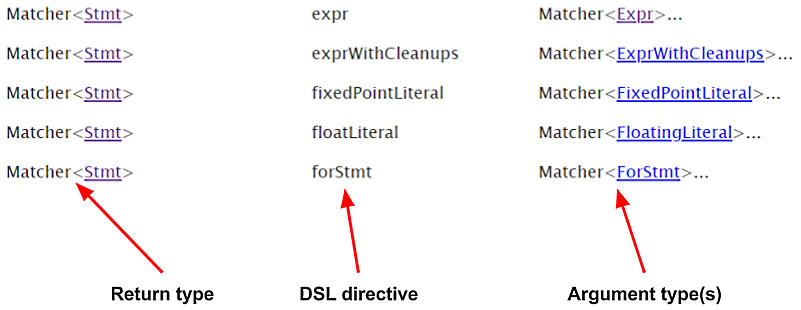
\includegraphics[width=0.9\textwidth]{content/2/chapter7/images/4.png}\\
图7.4 - ASTMatcher DSL参考的一部分
\end{center}

虽然这个表只是普通API引用的简化版本,但它已经展示了如何搜索候选指令。例如,现在了解了\texttt{forStmt(…)}可以接受0个或多个\texttt{Matcher<forStmt>},这样急救可以在这个表中搜索返回\texttt{Matcher<forStmt>}或\texttt{Matcher<(forStmt的父类)>}的指令,例如:\texttt{Matcher<stmt>}。本例中,我们可以快速地找到\texttt{hasCondition}、\texttt{hasBody}、\texttt{hasIncrement}或\texttt{hasLoopInit}作为候选指令(当然,也可以使用许多其他返回\texttt{Matcher<stmt>}的指令)。

当执行模式匹配时,不仅想知道一个模式是否匹配,还想获得匹配的AST节点。在ASTMatcher的上下文中,DSL指令只检查AST节点的类型。如果想要检索(部分)匹配的具体AST节点,可以使用\texttt{bind(…)}。下面是一个例子:

\begin{lstlisting}[style=styleCXX]
forStmt(
  hasCondition(
    expr().bind("exit_condition")));
\end{lstlisting}

这里,使用\texttt{expr()}作为通配符模式来匹配\texttt{expr}节点。这个指令还调用\texttt{bind(…)}来将匹配的\texttt{Expr} AST节点与\texttt{exit\_condition}的名称相关联。

然后,在前面介绍的\texttt{MatchCallback}中,我们可以使用以下代码检索绑定节点:

\begin{lstlisting}[style=styleCXX]
…
void run(const MatchFinder::MatchResult &Result) override {
	cons auto& Nodes = Result.Nodes;
	const Expr* CondExpr = Nodes.getNodeAs<Expr>
	("exit_condition");
	// Use `CondExpr`…
}
\end{lstlisting}

\texttt{getNodeAs<…>(…)}函数试图获取给定名称下绑定的AST节点,并将其转换为模板参数建议的类型。

注意,这里允许以相同的名称绑定不同的AST节点,这种情况下,在MatchCallback::run中,只显示最后一个有界的节点。

\hspace*{\fill} \\ %插入空行
\noindent
\textbf{合二为一}

现在已经了解了模式匹配DSL语法和如何使用ASTMatcher遍历AST,让我们把这两件事放在一起。

假设我们想知道一个简单的\texttt{for}循环(循环索引从0开始,每次迭代递增1,以一个整数为界)在函数中的迭代次数——也称为\texttt{trip count}:

\begin{enumerate}
\item 首先,必须编写以下代码来进行匹配和遍历:

\begin{lstlisting}[style=styleCXX]
auto PatExitCondition = binaryOperator(
                           hasOperatorName("<"),
                           hasRHS(integerLiteral()
                           .bind("trip_count")));
auto Pattern = functionDecl(
                  compountStmt(hasAnySubstatement(
               forStmt(hasCondition(PatExitCondition)))));
               
MatchFinder Finder;
auto* Callback = new MyMatchCallback();
Finder.addMatcher(traverse(TK_IgnoreUnlessSpelledInSource,
                           Pattern), Callback);
\end{lstlisting}

前面的代码片段还展示了模块化DSL模式的情况。可以创建单独的模式,只要它们兼容,可以根据需要组合它们。

最后,\texttt{MyMatchCallback::run}是这样的:

\begin{lstlisting}[style=styleCXX]
void run(const MatchFinder::MatchResult &Result) override
{
	const auto& Nodes = Result.Nodes;
	const auto* TripCount =
	Nodes.getNodeAs<IntegerLiteral>("trip_count");
	if (TripCount)
	TripCount->dump(); // print to llvm::errs()
}
\end{lstlisting}

\item 在此之后,可以使用\texttt{Finder}在AST上匹配所需的模式(通过调用\texttt{MatchFinder::match}或\texttt{MatchFinder::matchAST},或通过使用\texttt{MatchFinder::newASTConsumer}创建一个\texttt{ASTConsu\\mer})。匹配的行程计数将打印到\texttt{stderr},例如:输入的源代码是\texttt{for (int i = 0; i < 10; ++i) \{…\}},输出结果将是10。
\end{enumerate}

本节中,我们了解了Clang如何构造AST,如何在内存中表示Clang AST,以及如何使用ASTMatcher来帮助开发人员进行AST模式匹配。有了这些知识,在下一节中,我们将展示如何创建一个AST插件,这是将自定义逻辑注入到Clang编译管道最简单的方法。





















